\documentclass{article}%
\usepackage[T1]{fontenc}%
\usepackage[utf8]{inputenc}%
\usepackage{lmodern}%
\usepackage{textcomp}%
\usepackage{lastpage}%
\usepackage[head=40pt,margin=0.5in,bottom=0.6in]{geometry}%
\usepackage{graphicx}%
%
\title{\textbf{Arreaza espera que la UE "recupere el equilibro" con respecto a Venezuela}}%
\author{AVN}%
\date{07/03/2019}%
%
\begin{document}%
\normalsize%
\maketitle%
\textbf{URL: }%
http://www.eluniversal.com/politica/34993/arreaza{-}espera{-}que{-}la{-}ue{-}recupere{-}el{-}equilibro{-}con{-}respecto{-}a{-}venezuela\newline%
%
\textbf{Periodico: }%
EU, %
ID: %
34993, %
Seccion: %
politica\newline%
%
\textbf{Palabras Claves: }%
NO\_TIENE\newline%
%
\textbf{Derecho: }%
2.1%
, Otros Derechos: %
\newline%
%
\textbf{\textit{El canciller pidió a la Unión Europea reconsiderar "sus posiciones de permanente interferencia en nuestros asuntos internos, su clara alineación con la estrategia de agresión de Washington"}}%
\newline%
\newline%
%
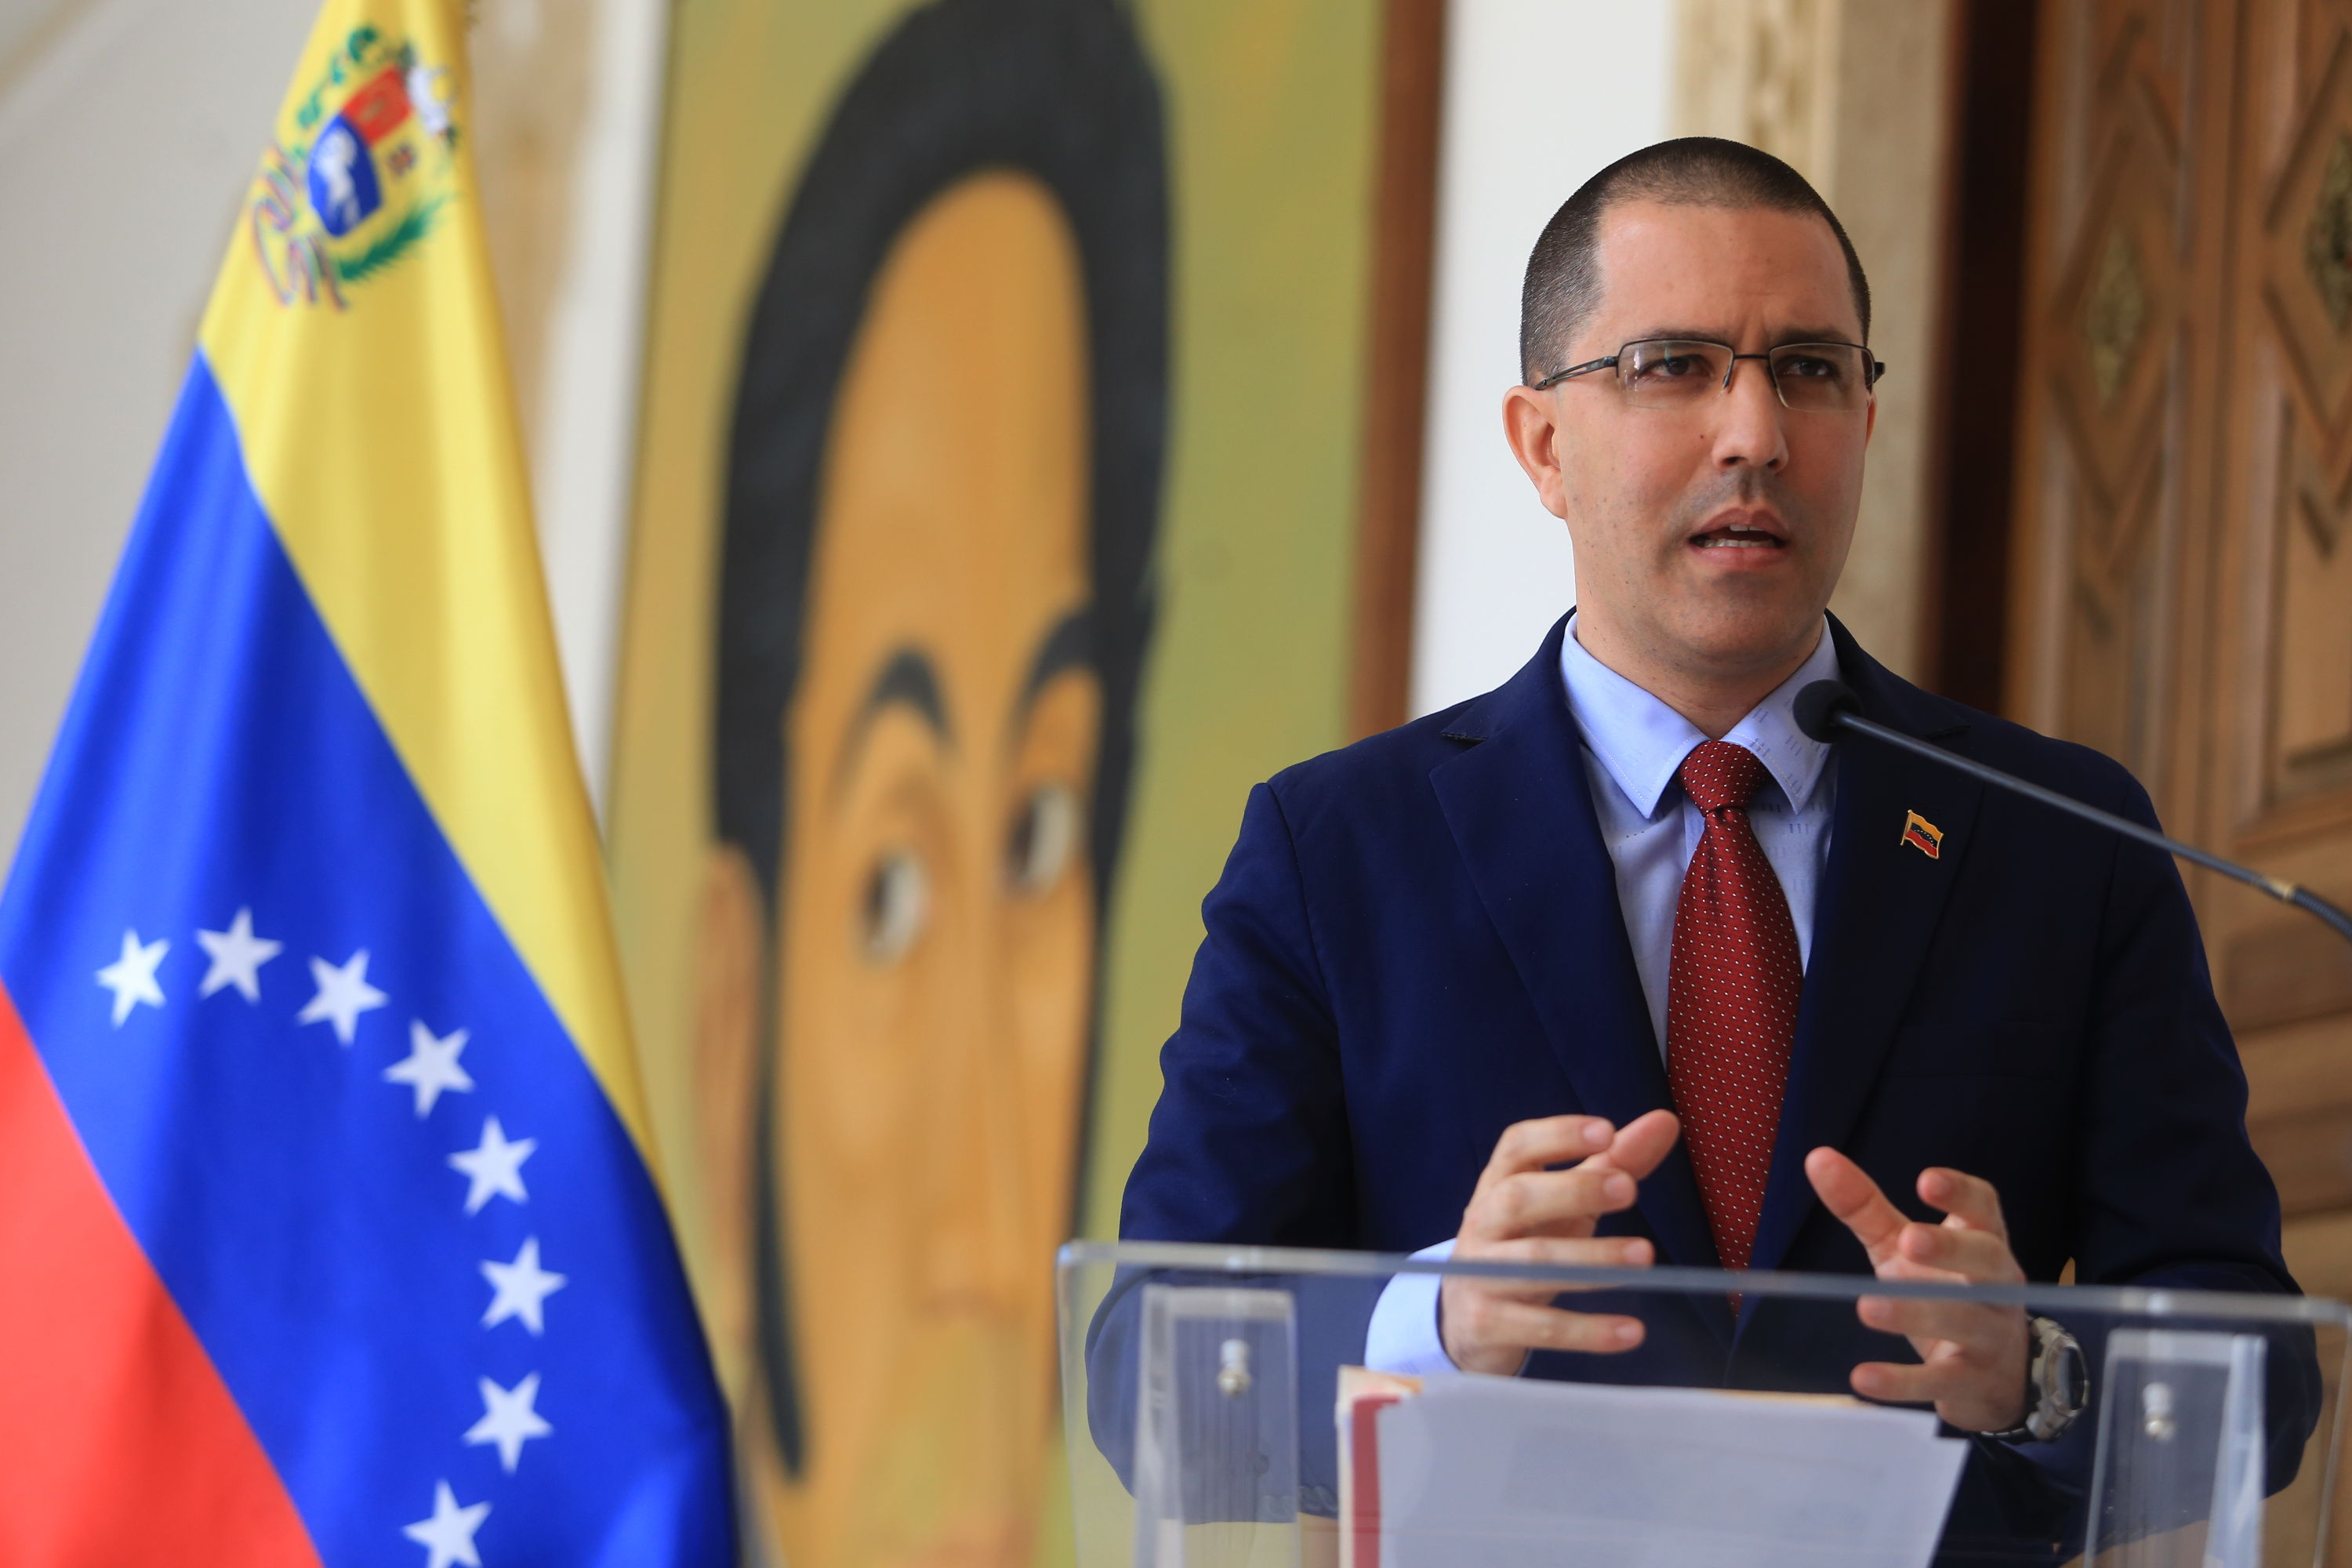
\includegraphics[width=300px]{EU_34993.jpg}%
\newline%
%
Caracas.{-}El ministro de Relaciones Exteriores, Jorge Arreaza, llamó a la Unión Europea (UE) a reconsiderar su posición de "interferencia" en los asuntos internos del país a propósito de la expulsión del embajador alemán del territorio venezolano.%
\newline%
%
"Venezuela espera que la Unión Europea recupere el EQUILIBRIO y RECONSIDERE sus posiciones de permanente interferencia en nuestros asuntos internos, su clara alineación con la estrategia de agresión de Washington y su apoyo a los actos inconstitucionales de la oposición extremista" escribió Arreaza en Twitter.%
\newline%
%
Más temprano, la UE lamentó~la decisión del Gobierno de Nicolás Maduro de expulsar al embajador alemán del país y dijo esperar que Caracas lo "reconsidere".%
\newline%
%
"Lamentamos el hecho de que el embajador alemán en Venezuela se vea obligado a abandonar el país en un contexto político tenso y complejo", dijo en rueda de prensa la vocera de la diplomacia europea, Maja Kocijancic.%
\newline%
%
El Gobierno de Maduro ordenó el miércoles al embajador alemán, Daniel Kriener, abandonar el país en 48 horas por "recurrentes actos de injerencia en los asuntos internos", por su respaldo al líder opositor Juan Guaidó.%
\newline%
%
\end{document}